\subsection*{Problema 06}

\textbf{Enunciado:} Calcular la integral:
\begin{align*}
\int \dfrac{\sqrt{x}}{x - 1} \, dx
\end{align*}

\textbf{Solución:} Siguiendo la indicación, 
realizamos el cambio de variable:
\begin{align*}
u &= \sqrt{x}, \quad x = u^2 \\
dx &= 2u \, du
\end{align*}

Sustituyendo en la integral original, 
obtenemos:
\begin{align*}
\int \dfrac{\sqrt{x}}{x - 1} \, dx &= \int \dfrac{u}{u^2 - 1} (2u \, du) \\
&= \int \dfrac{2u^2}{u^2 - 1} \, du
\end{align*}

Dado que el grado del numerador es igual 
al del denominador, dividimos la fracción 
algebraica o reescribimos el integrando:
\begin{align*}
\dfrac{2u^2}{u^2 - 1} &= \dfrac{2u^2 - 2 + 2}{u^2 - 1} \\
&= 2 + \dfrac{2}{u^2 - 1}
\end{align*}

Expandimos el término restante usando 
fracciones parciales:
\begin{align*}
\dfrac{2}{(u-1)(u+1)} &= \dfrac{A}{u-1} + \dfrac{B}{u+1}
\end{align*}

Resolviendo para los coeficientes, 
encontramos que $A = 1$ y $B = -1$. 
Entonces, la integral se descompone en:
\begin{align*}
\int \left( 2 + \dfrac{1}{u-1} - \dfrac{1}{u+1} \right) du
\end{align*}

Integramos término a término:
\begin{align*}
&= 2u + \ln|u-1| - \ln|u+1| + C \\
&= 2u + \ln\left|\dfrac{u-1}{u+1}\right| + C
\end{align*}

Finalmente, regresamos a la variable 
original $x$ sustituyendo $u = \sqrt{x}$:
\begin{align*}
= 2\sqrt{x} + \ln\left|\dfrac{\sqrt{x}-1}{\sqrt{x}+1}\right| + C
\end{align*}

\begin{figure}[H]
	\centering
	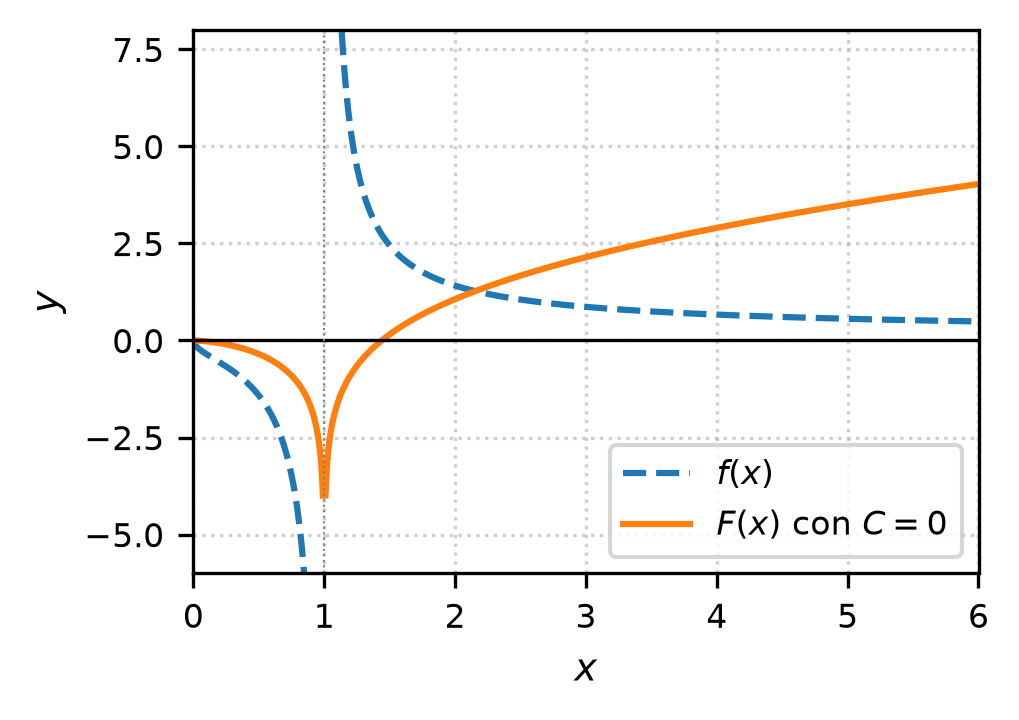
\includegraphics[width=\columnwidth]{semana_05/graficas/SEM05_P06_grafica.png}
	\caption{Representación gráfica de $f(x)$ y su antiderivada $F(x)$ evaluada para la constante de integración $C = 0$ (Problema 06).}
	\label{fig:problema06}
\end{figure}
